\chapter{Project Management}
This chapter describes the planning of this project in terms of scope, schedule, cost and risk.
The execution and deviations are shown at the end of this chapter.

\section{Scope}
\label{sec:scope}
The system has three parts: the \flangobe, the \flangofe (with the \se) both at Basestation, and the content application in the robots (the robot's \cm \fref{fig:system-overview}).

\begin{figure}[htb]
    \centering
    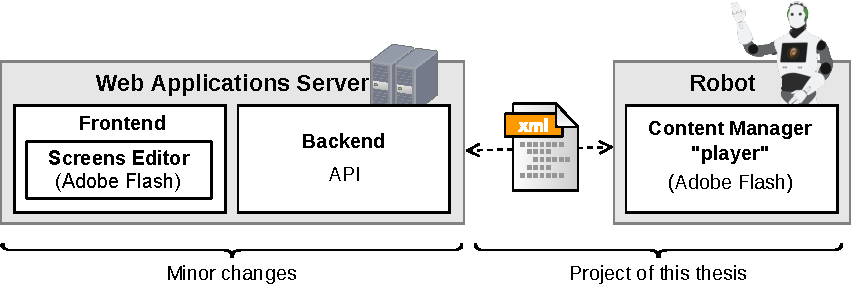
\includegraphics{figures/intro-system-overview.pdf}
    \caption{Boundaries and context of this project}
    \label{fig:system-overview}
\end{figure}

This project reengineers the robot's \cm with web technologies but not the back-end and front-end, that remain in Django and \flash.
The input of the new \cm are content applications, generated with the \se . The output is the screen rendered with web elements.
Content applications have configuration files that define the theme, the location of binary resources (images, videos, etc), the default language and other settings. 
This project can read and use the configuration files.
This project accepts valid syntax generated with the \se for a comprehensive set of components (\texttt{back-button}, \texttt{base-button}, \texttt{image}, \texttt{video}...) and their properties (\texttt{width}, \texttt{x}, \texttt{y}, \texttt{background}...), and generates \ac{HTML5} that displays them as they are defined in templates.

Developing an intense testing strategy is part of this project.
The final artifact is this master's thesis that describes the system and the rationale that guides all decisions.

\section{Schedule}
This project has 4 phases that match the 4 typical groups of processes: initiating, planning, executing (and monitoring + control) and closing.
The execution has 3 deliverables: viability and proof of concept, iteration 1 (basic program) and iteration 2 (extended program).

\subsection*{Phase 1: Initiating}
\paragraph{April, 1 -- April 4}
The initiating processes determine the goals of the project and the scope.
This stage was partially done before the beginning of this thesis to ensure its viability in the company.
It was agreed that the project would reengineer the current system using web technologies (see \fref{sec:scope})

\subsection*{Phase 2: Planning}
\begin{sidewaysfigure}[htb]   
    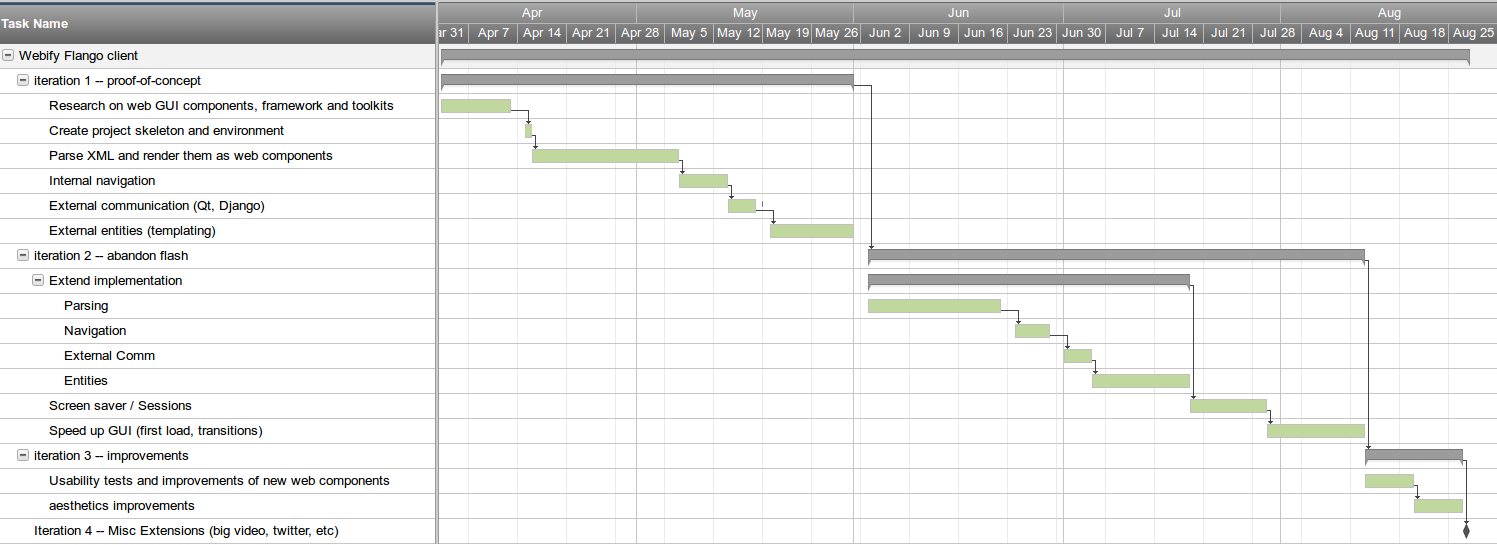
\includegraphics[width=\textwidth]{figures/plan-gantt-orig}
    \caption{Original Gantt Chart}
    \label{fig:plan-gantt}    
\end{sidewaysfigure}

\paragraph{April, 5 -- April 6}
The first draft of the plan is a rough estimation of the tasks length and a definition of the big milestones.
Because there is only one engineer there are no concurrent tasks and free floats are always zero.
Other activities of this phase include an estimation of the resource requirements for upcoming tasks, developing the budget (\fref{sec:budget}) and risk planning (\fref{sec:risk}).
See the Gantt chart in \fref{fig:plan-gantt}.

\subsection*{Phase 3: Execution}
\paragraph{April, 7 -- August 28}
The execution phase focuses on building the product. 
A web engineering process should be incremental, with frequent changes and short iterations \cite{Kappel:2006}.

\begin{table}[htb]
    \centering
    \begin{tabular}{| l | p{11cm} |}
    \hline
    Milestone & Deliverables \\
    \hline
    Proof of concept & Research on frameworks and tools to develop the project. Choose one. Build a minimal working example to illustrate key aspects of the project. \\ \hline
    Iteration 1 & Build a prototype comprehensive in number of features but simple in the implementation to validate the technology. \\ \hline
    Iteration 2 & Extend the prototype of Iteration 1 to complex cases. \\
    \hline
    \end{tabular}
    \caption{Milestones and deliverables of the execution phase}
    \label{tab:milestones}
\end{table}

This phase has 3 big milestones, one per iteration (\fref{tab:milestones}). 
The outcome of each iteration is a product with a set of stable features and the corresponding unit tests which, in turn, serve for the purpose of documentation.

\subsection*{Phase 4: Closing}
\paragraph{August, 29 -- September 14}
Prepare package with a stable set of features, presentation and documentation.

\FloatBarrier

\section{Cost}
\label{sec:budget}
The estimated length of the project is $95 days \times 8 \euro{} \times 8 hours = 6080 \euro{} $

\begin{table}[ht]
    \centering
    \begin{tabular}{| l | l |}
    \hline
    Labour & 6720\euro{} \\ \hline
    \multirow{3}{*}{Hardware} 
        & Desktop Computer (amortized) 250\euro{} \\ % check this
        & 22 Monitor (amortized) 50\euro{} \\
        & Reem H3 testing time 150\euro{} \\ \hline   
    \multirow{2}{*}{Software}
        & JetBrains WebStorm license 89.10\euro{} \\ % check this    
        & GNU/Linux 0\euro{} \\ \hline
     Overall & 6619.10\euro{} \\ 
     \hline
    \end{tabular}
    \caption{Budget}
    \label{tab:budget}
\end{table}

There are some infrastructure related costs excluded from the budget because they are part of the office maintenance monthly expenses.
This is the case of subversion servers, network, power, backups, etc. 

\section{Risk Analysis}
\label{sec:risk}
\begin{risk}
{Schedule: deviation}
{There might be urgent needs in the company, like demos to potential customers or hot bugs related to content applications}
{Some of the needs are unpredictable. However, preventive maintenance and good documentation of bugs in tickets can reduce the chances that this risk will occur.}
{Do the urgent task and reschedule the project}
\end{risk}

\begin{risk}
{Resources: deviation}
{The engineer might have to dedicate resources to other tasks in the company non-related to this project.}
{Coordinate action monthly with the managers and track deviations and progress weekly. Avoid dedicating less than 50\% of time to this project.}
{Limit scope and extend deadlines to have the expected number of hours dedicated to this project.}
\end{risk}

\begin{risk}
{Resources: infrastructure crash}
{The development system might die}
{Use version control systems and do frequent and small commits. Delegate backups to the IT team.}
{Restore backups}
\end{risk}

\begin{risk}
{Resources: testing environment not available}
{Most of the testing can be done with regular computers. However, final tests have to be conducted with real hardware: ReemH3-1 or 2 and Reem-H2, which are frequently booked to go on tour, perform shows, demos or development.}
{Book 3 days in advance if testing is critical. }
{Share the robot with a team that doesn't need the media computer of the robot, where this project is hosted.}
\end{risk}

\begin{risk}
{Personnel: Application expert leaves the project}
{There is only one application expert that can leave the company. Nobody else has advanced knowledge on the internals of the current implementation.}
{Build a common agenda with the expert and document critical and complex parts of the current application. Find experts in similar technology in the team}
{Reach him on-line, hire him as consultant, take conflicting features out of the scope of the project.}
\end{risk}

\begin{risk}
{Quality: critical use cases not implemented}
{One or more critical use cases can not be implemented}
{Verify that the technology allows implementing them. Build a prototype. }
{Find a workaround. Assess the importance of the affected use cases and adapt to change: decide if changing the specification of the use case will fix this.}
\end{risk}

\begin{risk}
{Quality: look and feel of the current theme can't be implemented}
{The current look and feel and interaction is designed for Adobe Flash. It might not suit the way web technology works.}
{Verify that the technology allows it with a prototype.}
{Change the external design to balance the needs of the technology and the customer}
\end{risk}

\begin{risk}
{Scope: Non-intuitive implementation with web technology}
{Current implementation is designed for Adobe Flex. Some of the use cases to implement might not fit well with the new technology}
{Analyse and discuss use cases with the author of the old implementation}
{Explore ways to change the implementation of the use case in the Screens Editor (which generates the input for the new program) to fit in the new design}
\end{risk}

\begin{risk}
{Inadequate technology}
{The chosen technology is inadequate: it doesn't allow a complete reengineering of the application (100\% of chosen use cases), performance is more than 10\% lower, it is not reliable and fails in more than 3\% of action executions}
{Assess at least 2 solutions before implementing a prototype. Implement a prototype with basic cases of at least each critical feature.}
{Stop the development and evaluate a different technology.}
\end{risk}

\begin{risk}
{Tool: Flango or \se do not perform as advertised}
{The current implementation of the backend or the screens editor might have bugs.
Some undocumented features or \ac{XML} elements might be misleading (e.g. The normal behaviour for the QR component is generating a QR code. \lstinline$<ui type="qr" src="path">$ does not generate a QR code, but embeds an image that already exists instead.) }
{Contact the application expert before implementing the feature.}
{Fix the backend (Python) or ask/hire the application expert to fix the screens editor (\flash)}
\end{risk}

\begin{risk}
{Angular or dependencies do not perform as advertised \footnote{Added after specifications were defined}}
{The chosen framework and libraries have young maturity and might contain bugs, be subject to rapid changing cycles and new versions might break older versions}
{Use stable versions}
{Investigate the bug, isolate it, create a minimal full working example and, if possible, open a pull request with a fix in Github or notify the error to the project managers.}
\end{risk}

\FloatBarrier

\section{Execution}
The project was planned initially to start on April 4 and end on September 1 with full-time dedication: 760h.
However, some situations caused a first delay and the ending day was pushed to October 10.
Another delay appeared and the final date was moved to December 18.
the overall number of hours remained approximately the same, 870h (+14\%).
Delays were caused by changes in the dedication time (with some weeks working only 20\% of the time on this project) or the appearance of risks.
This section summarises the execution of the project, the risks that appeared and the actions taken, the delays and the final result.

\subsection*{Scope}
The project had initially 2 iterations (\fref{tab:milestones}).
Whereas the first iteration was completed in time, in the second iteration entities were removed from the scope in order to deliver the project in time.
Parsing of deprecated components was also removed from the scope.

\subsection*{Risks}
\begin{itemize}
\item \textbf{Schedule and resources: deviation}. The company had urgent tasks and it was impossible to work full-time on this project. 
Among other delays, development was stopped for 2 weeks in June, 4 days in late July, and one week per month until December.
The development finished on the last week of November and this document was finished on December 8.
The solution was rescheduling all iterations and cutting the scope.
\item \textbf{Personnel: Application expert leaves the project}. The engineer that developed the old system left the company in September. Since then, only minor bugs have appeared and they have been fixed without contacting him. In September he had documented a big part of the project.
\end{itemize}

\subsection*{Cost}
The final length of the project is $109 days \times 8 \euro{} \times 8 hours = 6976 \euro{} $
\begin{table}[ht]
    \centering
    \begin{tabular}{| l | l |}
    \hline
    Labour & 6976\euro{} \\ \hline
    \multirow{3}{*}{Hardware} 
        & Desktop Computer (amortized) 250\euro{} \\ % check this
        & 22 Monitor (amortized) 50\euro{} \\
        & Reem H3 testing time 150\euro{} \\ \hline   
    \multirow{2}{*}{Software}
        & JetBrains WebStorm license 89.10\euro{} \\ % check this    
        & GNU/Linux 0\euro{} \\ \hline
     Overall & 7515.10\euro{} \\ 
     \hline
    \end{tabular}
    \caption{Final cost}
    \label{tab:final-cost}
\end{table}